\documentclass[12pt,spanish]{article}
\usepackage[spanish]{babel}
\usepackage{graphicx}
\usepackage{amsmath}
\usepackage{subcaption}
\usepackage{adjustbox}
\usepackage{multirow}
\usepackage[hidelinks]{hyperref}
\usepackage{caption}
\usepackage{amsthm}
\usepackage{multicol}
\usepackage[outputdir=build]{minted}
\usepackage{float}
\usepackage{titling}
\usepackage{soul}
\usepackage{listings}
\usepackage{array}
\graphicspath{ {./img/} {../../LaTeX/img/}}
\selectlanguage{spanish}
\usepackage[utf8]{inputenc}
\usepackage{graphicx}
\usepackage[a4paper,left=3cm,right=2cm,top=2.5cm,bottom=2.5cm]{geometry}


\title{Arquitectura de Computadores}
\setlength{\droptitle}{10em}
\author{Carlos Sánchez Páez}

\makeindex
\begin{document}


\begin{titlepage}

\newlength{\centeroffset}
\setlength{\centeroffset}{-0.5\oddsidemargin}
\addtolength{\centeroffset}{0.5\evensidemargin}
\thispagestyle{empty}

\noindent\hspace*{\centeroffset}
\begin{minipage}{\textwidth}

\centering

\includegraphics[width=0.9\textwidth]{logo_ugr.jpg}\\[1.4cm]

\textsc{ \Large Fundamentos de Ingeniería del Software1\\[0.2cm]}
\textsc{GRADO EN INGENIERÍA INFORMÁTICA}\\[1cm]

{\Huge\bfseries Resumen del temario\\}
\end{minipage}

\vspace{1.5cm}
\noindent\hspace*{\centeroffset}
\begin{minipage}{\textwidth}
\centering

\textbf{Autor}\\ {Carlos Sánchez Páez}\\[2.5ex]

\includegraphics[width=0.3\textwidth]{etsiit_logo.png}\\[0.1cm]
\vspace{1.5cm}

\includegraphics[width=0.2\textwidth]{lsi.png}\\[0.1cm]
\vspace{1cm}
\textsc{Escuela Técnica Superior de Ingenierías Informática y de Telecomunicación}\\
\vspace{1cm}
\textsc{Curso 2017-2018}
\end{minipage}
\end{titlepage}
\thispagestyle{empty}
\newpage
\tableofcontents{}
\listoffigures
\thispagestyle{empty}
\newpage

\section{Tema 1. Introducción a la Ingeniería del Software}

\subsection{El producto Software}

\subsubsection{Definición de Software}

El software se puede definir de varias formas:
\begin{itemize}
\item Programa o conjunto de programas de cómputo que incluye datos, procedimientos y pautas que permiten realizar distintas tareas en un sistema informático.
\item Transformador de información, para lo que adquiere, gestiona, modifica, produce o transmite esa información.
\end{itemize}

\subsubsection{Tipos de software}

Podemos clasificar el software en varios tipos:
\begin{enumerate}
	\item Por \emph{campo de aplicación}:
		\begin{enumerate}
			\item Software de \textbf{sistemas}.
			\item Software de \textbf{aplicaciones}.
			\item Sotware de \textbf{programación}.
		\end{enumerate}
	\item Por \emph{tipo de licencia}:
		\begin{enumerate}
			\item Según derechos de autor
				\begin{enumerate}
					\item Software de \textbf{código abierto}.
					\item Software de \textbf{código cerrado}.
					\item Software de \textbf{dominio público}.
				\end{enumerate}
			\item Según su destinatario
				\begin{enumerate}
					\item Usuario final (software \textbf{hecho a medida}).
					\item Para distribución (software \textbf{genérico}).
				\end{enumerate}
		\end{enumerate}
\end{enumerate}

\subsubsection{Características principales}

\begin{enumerate}
	\item El software es un producto lógico:
		\begin{enumerate}
			\item No se fabrica, sino que se desarrolla.
			\item No se estropea, sino que se deteriora.
		\end{enumerate}
	\item Crea modelos de la realidad.
	\item Está formado por múltiples piezas que deben encajar perfectamente.
\end{enumerate}

\subsubsection{Proceso de producción}

El proceso de producción del software está formado por las siguientes etapas:
\begin{enumerate}
	\item \textbf{Definición}. Debemos precisar lo que queremos desarrollar. Para ello debemos realizar varias tareas:
		\begin{itemize}
			\item Ingeniería de Sistemas.
			\item Ingeniería de Requisitos.
			\item Planificación de proyectos.
		\end{itemize}
	\item \textbf{Construcción}. Hemos de determinar cómo desarrollaremos el software. Depende de:
		\begin{itemize}
			\item Diseño del software.
			\item Generación del código.
			\item Prueba del software.
		\end{itemize}
	\item \textbf{Evolución}. Consiste en precisar las partes del software que cambiarán.
		\begin{itemize}
			\item Corrección.
			\item Adaptación.
			\item Mejora.
			\item Prevención.
		\end{itemize}
\end{enumerate}
\begin{figure}[H]
\centering
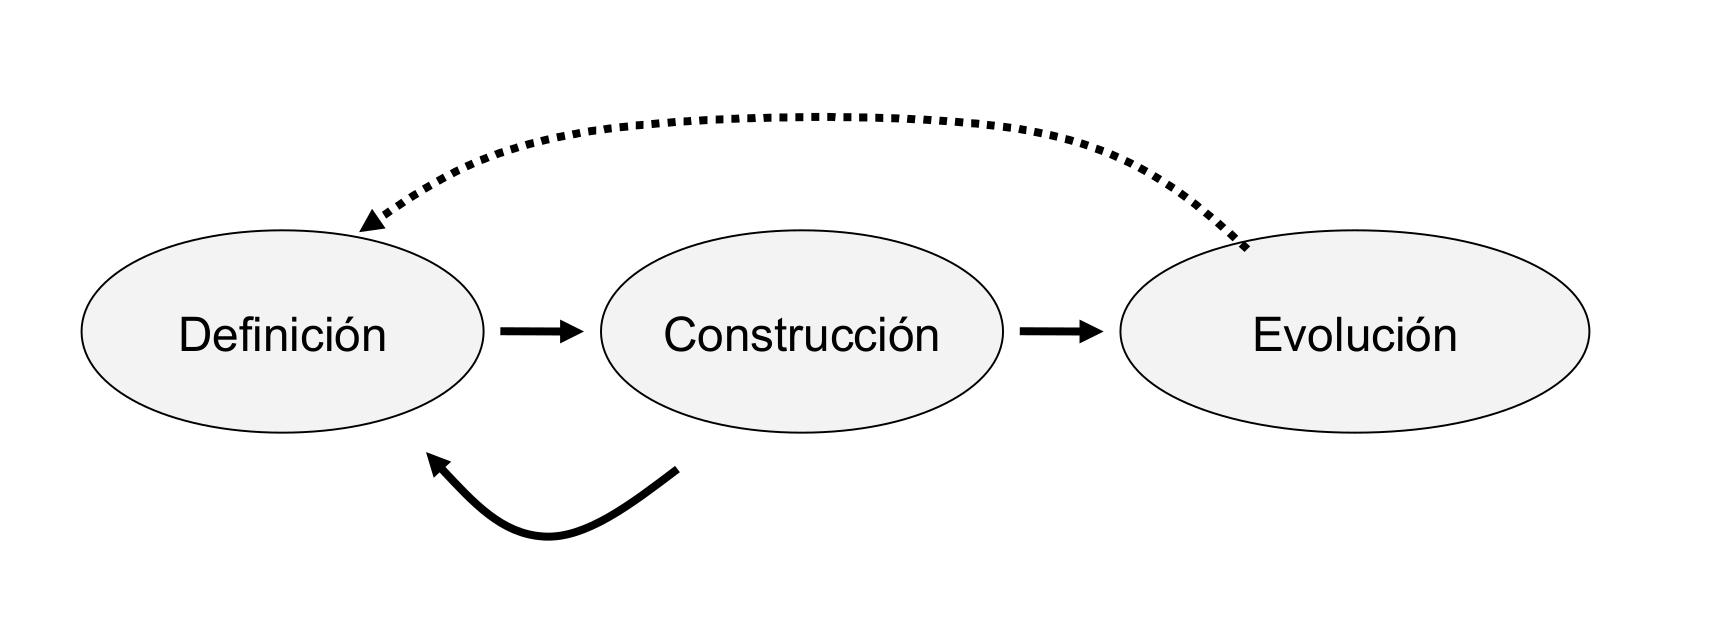
\includegraphics[scale=0.2]{proceso_produccion.png}
\caption{Etapas del proceso de producción del software.}
\end{figure}

\begin{figure}[H]
\centering
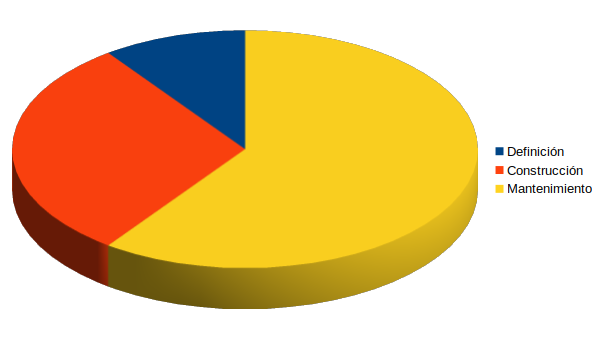
\includegraphics[scale=0.75]{esfuerzo_etapas.png}
\caption{Esfuerzo invertido en las distintas etapas.}
\end{figure}

\begin{figure}[H]
\centering
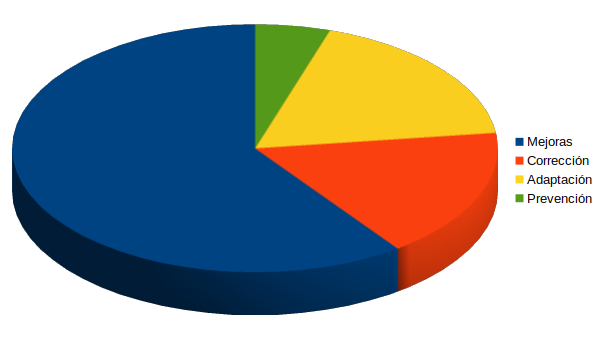
\includegraphics[scale=0.75]{esfuerzo_mantenimiento.png}
\caption{Esfuerzo invertido en las distintas etapas del mantenimiento.}
\end{figure}

\newpage

\subsubsection{Problemas en el desarrollo}

\begin{enumerate}
	\item \textbf{Comunicación} entre personas.
		\begin{figure}[H]
		\centering
		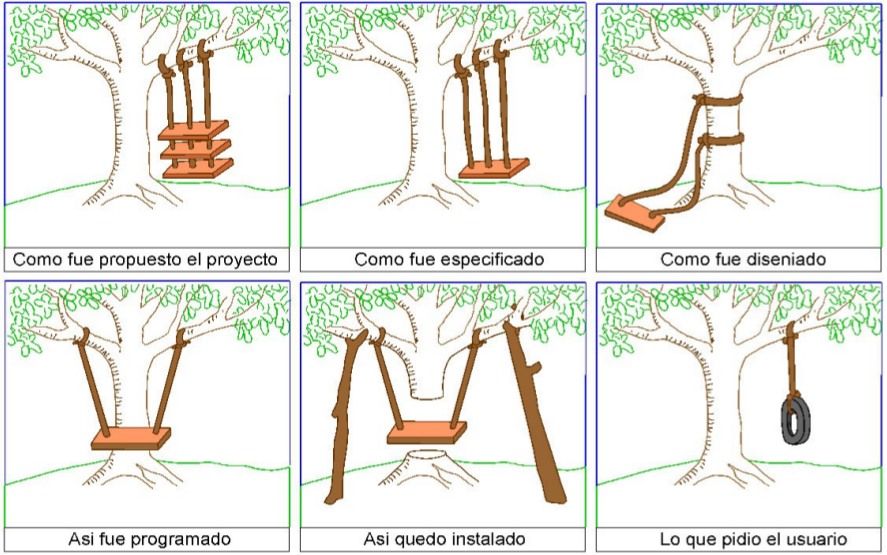
\includegraphics[scale=0.5]{problema_comunicacion.png}
		\caption{Problemas en la comunicación.}
		\end{figure}
	\item Incumplimiento de la \textbf{planificación}.
	\item Incorporación de \textbf{cambios} en etapas avanzadas.
		\begin{figure}[H]
		\centering
		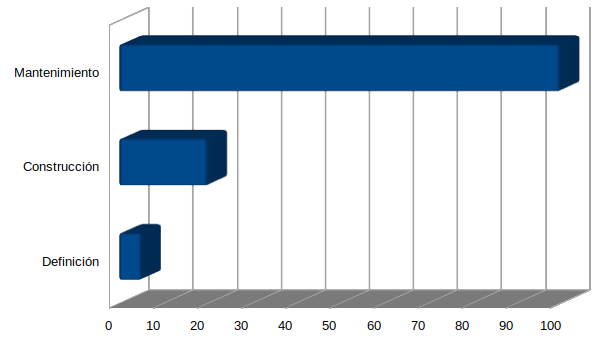
\includegraphics[scale=0.8]{impacto_cambio.png}
		\caption{Impacto del cambio en las distintas etapas.}
		\end{figure}
\end{enumerate}

\paragraph{Desastres ocasionados por sistemas software}
La mayoría de ellos tienen como causa pruebas deficientes, mala documentación, diseños pobres o inexistentes, mal estudio del problema, etc.

\subsection{Concepto de Ingeniería del Software}

La \emph{Ingeniería del Software} surgió por varias necesidades:
\begin{itemize}
	\item Mal funcionamiento (calidad).
	\item Mantenimiento del software existente.
	\item Demanda creciente del nuevo software.
	\item Adaptación a las nuevas tecnologías.
	\item Incremento de la complejidad.
\end{itemize}

\subsubsection{Definiciones de la Ingeniería del Software}

\begin{enumerate}
	\item Establecimiento de los principios y métodos de la ingeniería a fin de obtener software de modo rentable que sea fiable y trabahe en máquinas reales.
	\item Aplicación práctica del conocimiento científico en el diseño y construcción de programas de computadora y la documentación asociada y requerida para el desarrollo, operación y mantenimiento del programa.
	\item Estudio de los principios y métodos para el desarrollo y mantenimiento de sistemas software.
	\item Aplicación de un enfoque sistémico, disciplinado y cuantificable al desarrollo, operación y mantenimiento del software; es decir, aplicación de la ingeniería al software.
	\item Conjunto de teorías, métodos e instrumentos (tecnológicos y organizativos) que permitan construir sistemas software con las características de calidad deseadas.
	\item Disciplina de ingeniería que se interesa por todos los aspectos de la producción de software, desde las primerasa etapas de la especificación hasta el mantenimiento del sistema después de su puesta en operación.
\end{enumerate}

\subsubsection{Terminología usada en Ingeniería del Software}

\begin{itemize}
	\item \textbf{Sistema}. Conjunto de elementos relacionados entre sí y con el medio, que forman una unidad o un todo organizativo.
	\item \textbf{Sistema basado en computadora}. Conjunto o disposición de elementos organizados para cumplir una meta predefinida al procesar información.
		\begin{figure}[H]
		\centering
		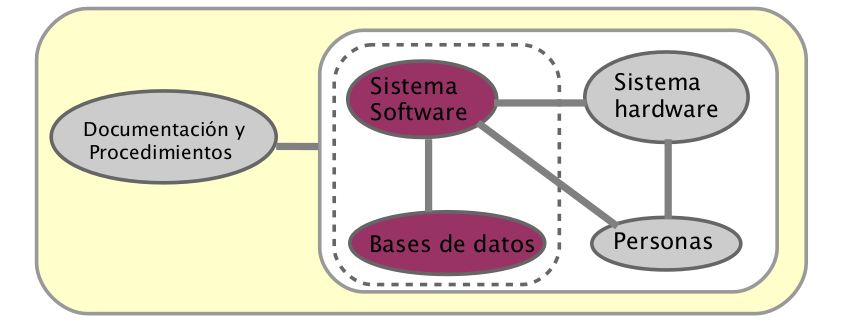
\includegraphics[scale=0.35]{sist_basado_comp.png}
		\caption{Sistema basado en computadora.}
		\end{figure}
	\item \textbf{Sistema Software}. Conjunto de piezas o elementos software relacionados entre sí y organizados en subsistemas.
		\begin{figure}[H]
		\centering
		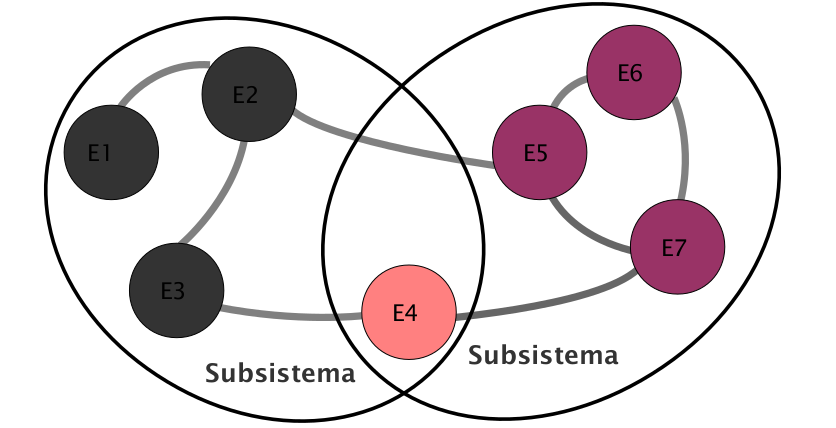
\includegraphics[scale=0.35]{sist_software.png}
		\caption{Sistema Software.}
		\end{figure}
	\item \textbf{Modelo}. Representación de un problema en un determinado lenguaje. De un mismo problema se pueden construir muchos modelos.
		\begin{figure}[H]
		\centering
		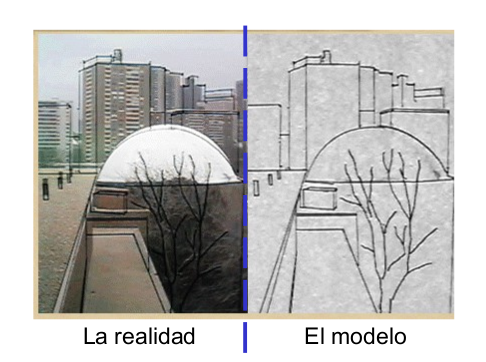
\includegraphics[scale=0.65]{modelo.png}
		\caption{Modelo.}
		\end{figure}
	\item \textbf{Principio}. Elementos que son adquiridos mediante el conocimiento. Determinan las características que debe poseer un modelo para ser una representación adecuada de un sistema.
	\item \textbf{Herramienta}. Instrumentos que permiten la representación de modelos.
	\item \textbf{Técnica}. Modo de utilización de las herramientas.
	\item \textbf{Heurísticas}. Conjunto de reglas empíricas que al ser aplicadas producen modelos que se adecuan a los principios. Ejemplo: \textit{No usar materiales flexibles para representar la maqueta de un edificio}.
	\item \textbf{Proceso}. Estructura que debe establecerse para la obtención eficaz de un producto de Ingeniería.
	\item \textbf{Método}. Proporciona la experiencia técnica para elaborar el producto software. Se basa en principios fundamentales e incluye actividades de modelado.
	
\end{itemize}

\subsection{Proceso de desarrollo del software}

\subsubsection{Concepto de proceso de desarrollo}

\begin{itemize}
	\item \textbf{Proceso de desarrollo del software}. Conjunto de \emph{actividades, acciones y tareas} que se realizan cuando va a crearse un producto o sistema software.
	\item \textbf{Actividad}. Busca el logro de objetivos amplios e independientes del tipo de aplicación a desarrollar y su complejidad.
	\item \textbf{Acción}. Conjunto de tareas que elaboran un producto importante como resultado.
	\item \textbf{Tarea}. Objetivo pequeño y bien definido que produce un resultado tangible.
\end{itemize}

Las actividades que se realizan pueden ser de varios tipos:

\begin{enumerate}
	\item \textbf{Estructurales}. Se dedican a obtener el producto:
		\begin{enumerate}
			\item \textbf{Comunicación}. Colaboración con el cliente para entender los objetivos y requisitos del proyecto.
			\item \textbf{Planificación}. Definición del plan de proyecto en el que se describen los riesgos probables, recursos adquiridos y productos obtenidos a la vez que se programan las actividades, acciones y tareas.
			\item \textbf{Modelado}. Representación mediante modelos del sistema porpuesto junto con la solución o soluciones apropiadas.
			\item \textbf{Construcción}. Generación de código y su prueba.
			\item \textbf{Despliegue}. Entrega al consumidor y evaluación por parte de éste, lo que sirve como retroalimentación para el equipo de desarrollo.
		\end{enumerate}

	\item \textbf{Sombrilla}. Se aplican a lo largo de todo el proceso. Se dedican a:
		\begin{enumerate}
			\item Seguimiento y control del proyecto.
			\item Administración del riesgo.
			\item Aseguramiento de la calidad.
			\item Revisiones técnicas.
			\item Mediciones de parámetros del proceso.
			\item Administración de la configuración.
			\item Administración de la reutilización.
			\item Preparación y producción del producto de trabajo.
		\end{enumerate}
	
\end{enumerate}

\subsubsection{Modelo general de proceso}
\begin{itemize}
	\item \textbf{Estructura del proceso}. Cada una de las actividades, acciones y tareas se encuadran dentro de una estructura que define su relación con el proceso y entre ellas.
		\begin{figure}[H]
		\centering
		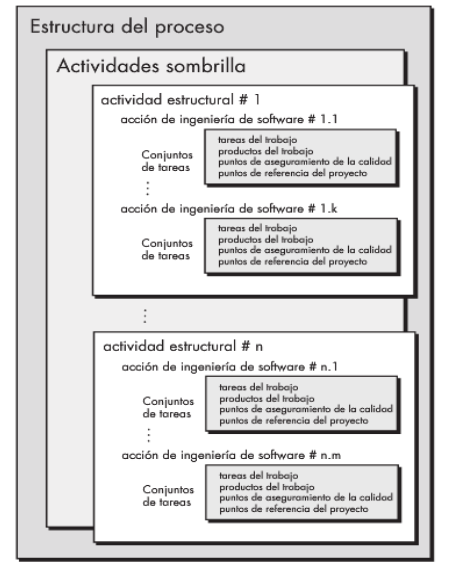
\includegraphics[scale=0.5]{estructura_proceso.png}
		\caption{Estructura del proceso.}
		\end{figure}	
	\item \textbf{Flujo del proceso}. Describe la forma en la que se organizan las actividades estructurales, acciones y tareas en los procesos con respecto a la secuencia y el tiempo.
		\begin{figure}[H]
			\centering
			\begin{subfigure}[H]{0.5\textwidth}
			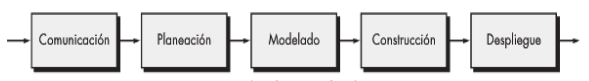
\includegraphics[width=\textwidth]{proceso_lineal.png}
			\caption{Flujo de proceso lineal.}
			\end{subfigure}
			\vskip 10pt
			\begin{subfigure}[H]{0.5\textwidth}
			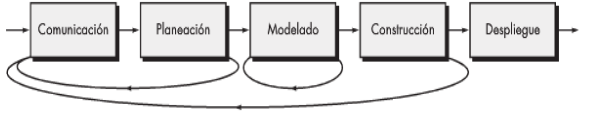
\includegraphics[width=\textwidth]{proceso_iterativo.png}
			\caption{Flujo de proceso iterativo.}
			\end{subfigure}
			
			\begin{subfigure}[H]{0.5\textwidth}
			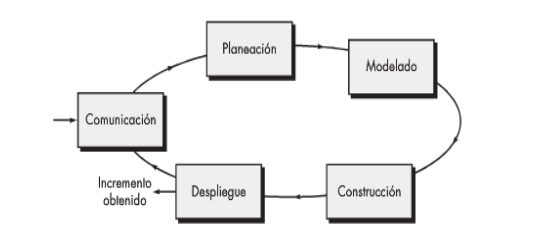
\includegraphics[width=\textwidth]{proceso_evolutivo.png}
			\caption{Flujo de proceso evolutivo.}
			\end{subfigure}
			\caption{Tipos de flujos de proceso.}
		\end{figure}
	\item \textbf{Acciones y tareas de las actividades estructurales}.
		\begin{enumerate}
			\item \textbf{Obtención de requisitos}. Obtención de información respecto a la acción que debe realizar el software.
			\item \textbf{Estimación y planificación del proyecto}. Estimar el tiempo y los costes del desarrollo del software.
			\item \textbf{Análisis de requisitos}. Documento en el que se especifica lo que debe hacer el sistema software.
			\item \textbf{Diseño}. Búsqueda de la solución. Descripción de los componentes, sus relaciones y funciones que le dan solución al problema.
			\item \textbf{Implementación}. Traducción del diseño a un lenguaje de programación entendible por una máquina.
			\item \textbf{Prueba del software}. Revisión y validación del código que se va desarrollando.
			\item \textbf{Evaluación y aceptación}. Evaluación del producto y aceptación por parte de los interesados en él.
			\item \textbf{Entrega y asistencia}. Sistema pasa a operar y se ofrece asistencia para su correcto funcionamiento.
		\end{enumerate}
\end{itemize}

\subsubsection{Tipos de modelos de proceso}

\begin{itemize}
	\item \textbf{Modelo en cascada}. Presenta una estructura secuencial y un flujo lineal. Sin embargo, los proyectos no suelen adecuarse a este modelo, es difícil expresar los requisitos a través de él al principio del proyecto y ofrece poca comunicación con el cliente, ya que hasta el final no hay un ejecutable que se pueda evaluar.
		\begin{figure}[H]
			\centering
			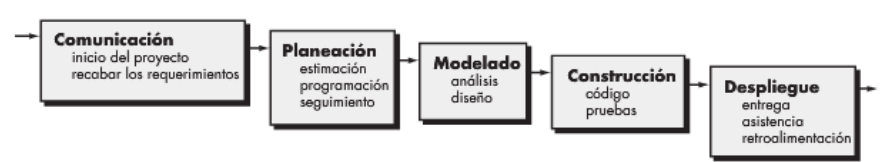
\includegraphics[scale=0.5]{modelo_cascada.png}
			\caption{Modelo en cascada.}
		\end{figure}
	\newpage
	\item \textbf{Modelo incremental}. Su estructura es secuencial mientras  que el flujo de proceso es lineal y paralelo entre incrementos.
			\begin{figure}[H]
			\centering
			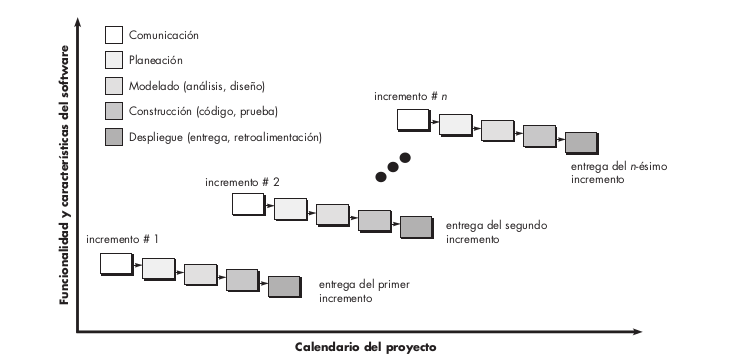
\includegraphics[scale=0.5]{modelo_incremental.png}
			\caption{Modelo incremental.}
		\end{figure}
	\item \textbf{Modelo evolutivo}. Es también iterativo. Nace como solución a varios factores, como un tiempo de entrega muy limitado o la necesidad de facilitar la incorporación de cambios. En cada iteración del proceso se obtiene un producto terminado y operativo. Sus características generales son:
	\begin{enumerate}
		\item Afrontan los riesgos altos (técnicos, de requisitos, etc.) tan pronto como sea posible.
		\item Retroalimentación temprana por parte del cliente.
		\item Manejo de la complejidad (pasos cortos y sencillos).
		\item El conocimiento adquirido durante una iteración de la evolución se puede usar en el resto de iteraciones.
		\item Involucra continuamente al usuario (evaluación, retroalimentación, afinamiento y refinamiento de requisitos, etc.).
	\end{enumerate}
	\newpage
	Hay dos tipos fundamentales de modelos evolutivos:
	\begin{enumerate}
		\item \textbf{Modelo de prototipos}. Un prototipo es una representación limitada de un producto que se utiliza para probar su diseño y comprender mejor el problema y sus posibles soluciones. Los prototipos pueden ser \emph{evolutivos} (productos finales) o \emph{desechables} (usados dentro de otros modelos de proceso).
		\begin{figure}[H]
		\centering
		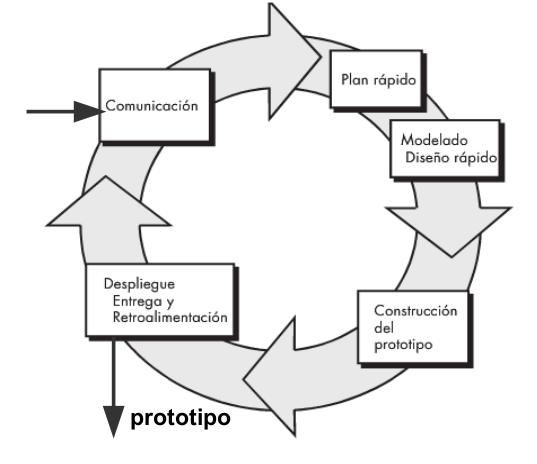
\includegraphics[scale=0.5]{modelo_prototipos.png}
		\caption{Modelo de prototipos}
		\end{figure}
	\end{enumerate}
	Este modelo se utiliza para:
	\begin{enumerate}
		\item Facilitar la obtención y validación de requisitos (\emph{desechable}).
		\item Estudios de viabilidad (\emph{desechable}).
		\item Propuestas de diseños alternativos (\emph{desechable}).
		\item En casos muy concretos como producto final (\emph{evolutivo}). 
	\end{enumerate}
	Presentan todas las características de los modelos evolutivos, aunque se les añaden algunos inconvenientes:
	\begin{itemize}
		\item Crear falsas expectativas por parte del cliente (\emph{desechable}).
		\item Puede que el prototipo \emph{desechable} se elabore con una metodología ineficiente y ésta se mantenga en el producto final.
	\end{itemize}
	\item \textbf{Modelo en espiral de Boehm}. Además de las características de los procesos iterativos, incluye otras más:
	\begin{enumerate}
		\item Se centra en el análisis de riesgo, construyendo prototipos para su estudio.
		\item La espiral puede continuar una vez que se entregue el momento para llevar a cabo el mantenimiento.
		\item Es adecuado para el desarrollo de sistemas a gran escala.
	\end{enumerate}
	Sus principales inconvenientes son que no es controlable y que requiere un equipo de desarrollo con gran experiencia en análisis de riesgo.
	\begin{figure}[H]
		\centering
		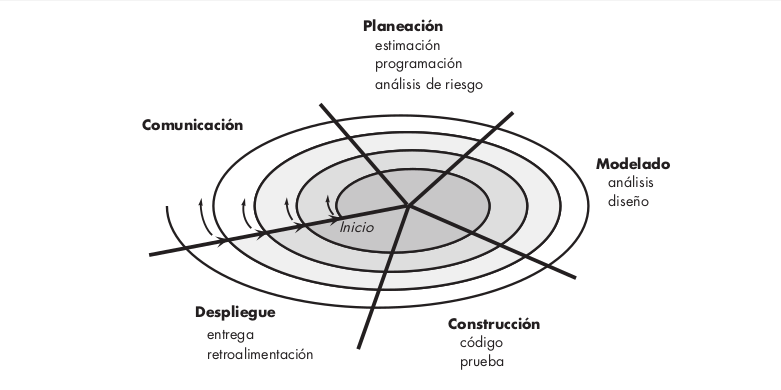
\includegraphics[scale=0.5]{modelo_espiral.png}
		\caption{Modelo en espiral de Boehm}
	\end{figure}
\end{itemize}

\subsubsection{Proceso unificado}
Es un modelo de proceso evolutivo y compuesto por cuatro fases:
\begin{itemize}
	\item Inicio o concepción.
	\item Elaboración.
	\item Construcción.
	\item Transición.
\end{itemize}
Estas etapas se reparten entre las actividades estructurales como podemos ver en el diagrama:

\begin{figure}[H]
			\centering
			\begin{subfigure}[b]{0.4\textwidth}
			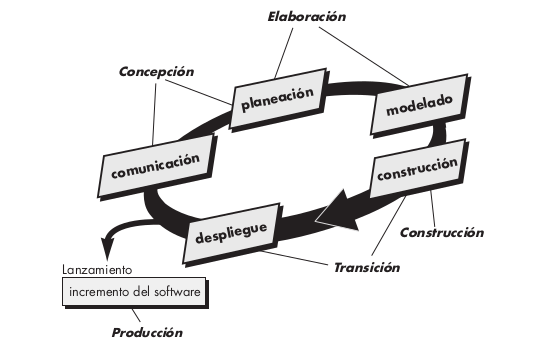
\includegraphics[width=\textwidth]{proceso_unificado.png}
			\end{subfigure}
			\quad
			\begin{subfigure}[b]{0.5\textwidth}
			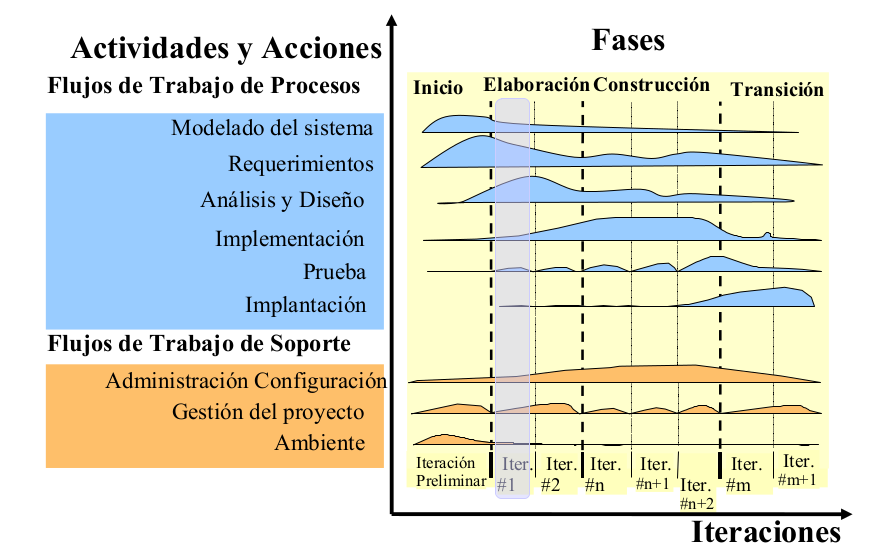
\includegraphics[width=\textwidth]{proceso_unificado_2.png}
			\end{subfigure}

			\caption{Proceso unificado.}
\end{figure}
\newpage
Además de las características de los modelos de proceso evolutivos, el proceso unificado incorpora las siguientes:
\begin{enumerate}
	\item Es un modelo de proceso adaptable a la complejidad y al tipo de sistema.
	\item Está centrado en la arquitectura, mostrando y decidiendo los distintos aspectos arquitectónicos de un sistema software en etapas tempranas. De esta forma pueden servir de base a las posteriores.
	\item Está dirigido por casos de uso, desarrollándose uno o varios en cada iteración. En iteraciones tempranas los casos de uso determinarán la arquitectura.
\end{enumerate}
\paragraph{Acciones y tareas en cada fase}
\begin{itemize}
	\item \textbf{Inicio}. Agrupa actividades tanto de comunicación del cliente como de planificación. Se propone una arquitectura aproximada para el sistema y se estudian numerosos factores (viabilidad, alcance, riesgos, etc.).
	\item \textbf{Elaboración}. Incluye actividades de comunicación y modelado de la arquitectura básica sobre la que se asentará la fase de construcción.
	\item \textbf{Construcción}. Se completan los modelos de requisitos y se implementan los elementos necesarios para completar el sistema. Según se van terminando los elementos, son probados e integrados al producto final. También se realizan pruebas de aceptación por parte del usuario.
	\item \textbf{Transición}. Consiste en asegurarse de que el sistema cumple con los requisitos especificados (mediante pruebas por parte de los usuarios). Además, se genera el material necesario para lanzar el producto al mercado.
\end{itemize}

\begin{figure}[H]
	\centering
	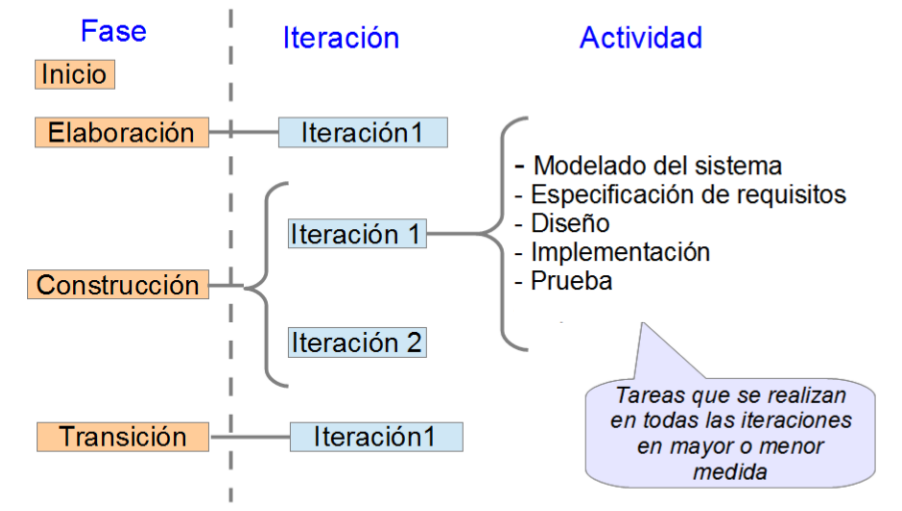
\includegraphics[scale=0.45]{proceso_unificado_ej.png}
	\caption{Ejemplo de Proceso Unificado}
\end{figure}

\subsubsection{Desarrollo Ágil}
En 2001, diecisiete expertos se preguntaron por qué muchos proyectos generaban menos valor del esperado, no se terminaban a tiempo, tenían problemas de calidad serios, etc. Tras ésto, elaboraron el \emph{Manifiesto el Desarrollo Ágil de Software} con el que intentaban dar solución a estos problemas.
\paragraph{Características del Desarrollo Ágil}
\begin{enumerate}
	\item Es un proceso iterativo e incremental, por lo que es evolutivo.
	\item Requiere entregas frecuentes y trabajo en equipo.
	\item Establece autonomía en el equipo de desarrollo.
	\item Exige revisiones y reuniones retrospectivas frecuentes.
\end{enumerate}
Sus beneficios son que se mejora la productividad y que se manejan mejor los riesgos.\\
Consta de varias técnicas:
\begin{itemize}
	\item Scrum
	\item XP (\emph{Extreme Programming})
	\item Programación en parejas.
	\item TDD (\emph{Test Driven Development})
\end{itemize}

\newpage

 
\section{Tema 2. Ingeniería de Requisitos}

\subsection{Introducción}

En 1995 se realizó el informe \emph{CHAOS} sobre los resultados que se obtuvieron en diversos proyectos software:
\begin{figure}[H]
\centering
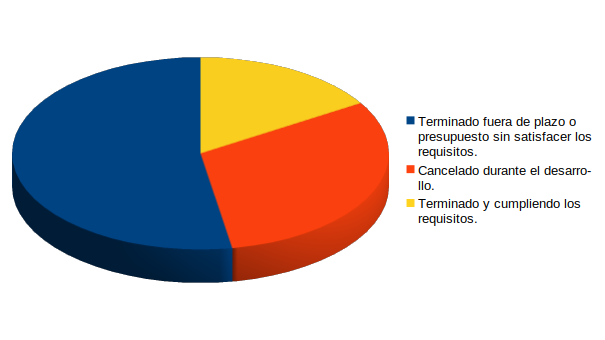
\includegraphics[scale=0.75]{informe_chaos.png}
\caption{Resultados del informe \emph{CHAOS}.}
\end{figure}

Los principales factores de fracaso son:

\begin{enumerate}
	\item Falta de información por parte de los usuarios.
	\item Especificación de requisitos incompleta.
	\item Continuos cambios de los requisitos.
	\item Pobres habilidades técnicas en la especificación de requisitos.
\end{enumerate}

La \textbf{Ingeniería de Requisitos} cubre las tareas y proporciona los mecanismos adecuados para:
\begin{itemize}
	\item Entender y analizar las necesidades del cliente.
	\item Evaluar la viabilidad de las necesidades.
	\item Negociar una solución razonable.
	\item Especificar la solución sin ambigüedades, confeccionando un documento que describa la solución acordada.
	\item Validar y analizar la especificación reflejada en el documento de especificación de requisitos, obteniendo el \emph{modelo de análisis}.
	\item Administrar y desarrollar los requisitos a lo largo del proceso de desarrollo.
\end{itemize}

El proceso de construcción de una \emph{especificación de requisitos} es iterativo. En él, partimos de las especificaciones iniciales imcompletas, poco claras y ambiguas y llegamos a especificaciones finales \textbf{completas, claras, documentadas y validadas}.









































































































\end{document}